\documentclass[11pt,a4paper]{article}

%----------------------------------------------------------------------------------------
%	PACKAGES & CONFIGURATION (Standard LaTeX Only - Zero External Templates)
%----------------------------------------------------------------------------------------
\usepackage[utf8]{inputenc}
\usepackage[T1]{fontenc}
\usepackage{lmodern}
\usepackage[left=0.6in, right=0.6in, top=0.6in, bottom=0.6in]{geometry}
\usepackage{xcolor}
\usepackage{graphicx}
\usepackage{amsmath}
\usepackage{fontawesome5}
\usepackage{academicons}
\usepackage{simpleicons}
\usepackage{enumitem}
\usepackage{tabularx}
\usepackage{microtype}
\usepackage{needspace}
\usepackage[pdftex,
    colorlinks=true,
    urlcolor=cvblue,
    linkcolor=cvblue,
    citecolor=cvblue,
    pdfauthor={Saptarshi Sadhu},
    pdftitle={Curriculum Vitae - Saptarshi Sadhu},
    pdfsubject={Academic Research CV}]{hyperref}

%----------------------------------------------------------------------------------------
%	COLOR PALETTE (Matching exact ModernCV Classic Blue Theme)
%----------------------------------------------------------------------------------------
\definecolor{cvblue}{RGB}{56, 115, 173}  % Classic ModernCV Blue (#3873AD)
\definecolor{cvdark}{RGB}{51, 51, 51}    % Soft Dark (#333333)
\definecolor{cvgray}{RGB}{127, 127, 127} % Hint Gray (#7F7F7F)

% Page Setup
\pagestyle{empty}
\setlength{\parindent}{0pt}
\setlength{\parskip}{0pt}

% Section Geometry Dimensions (3.6cm hint column for balanced dates and headers)
\newlength{\hintscolumnwidth}
\setlength{\hintscolumnwidth}{3.6cm}
\newlength{\separatorcolumnwidth}
\setlength{\separatorcolumnwidth}{0.4cm}
\newlength{\maincolumnwidth}
\setlength{\maincolumnwidth}{\dimexpr\textwidth-\hintscolumnwidth-\separatorcolumnwidth\relax}

% Custom Section Header Command with Orphan Prevention (\needspace + \nopagebreak)
\newcommand{\cvsection}[1]{%
  \par\vspace{10pt}%
  \needspace{5\baselineskip}%
  \phantomsection
  \noindent
  \begin{minipage}[t]{\hintscolumnwidth}
    \raggedleft
    \color{cvblue}\rule[0.3ex]{\linewidth}{3.5pt}%
  \end{minipage}%
  \hspace{\separatorcolumnwidth}%
  \begin{minipage}[t]{\maincolumnwidth}
    {\raggedright\fontsize{12.5}{14.5}\selectfont\bfseries\color{cvblue} #1}
  \end{minipage}%
  \par\nopagebreak\vspace{5pt}\nopagebreak%
}

% Standard Item Macro (Left Column: Date/Hint, Right Column: Content)
\newcommand{\cvitem}[2]{%
  \vspace{3pt}%
  \noindent
  \begin{minipage}[t]{\hintscolumnwidth}
    \raggedleft\small\bfseries\color{cvdark} #1
  \end{minipage}%
  \hspace{\separatorcolumnwidth}%
  \begin{minipage}[t]{\maincolumnwidth}
    \raggedright\sloppy\color{cvdark} #2
  \end{minipage}%
  \par\vspace{3pt}%
}

% Entry Macro for Roles & Experience
\newcommand{\cventry}[6]{%
  \vspace{4pt}%
  \noindent
  \begin{minipage}[t]{\hintscolumnwidth}
    \raggedleft\small\bfseries\color{cvdark} #1
  \end{minipage}%
  \hspace{\separatorcolumnwidth}%
  \begin{minipage}[t]{\maincolumnwidth}
    \raggedright\sloppy
    {\bfseries #2}%
    \ifx&#3&\else\\[1.5pt]\textit{#3}\fi%
    \ifx&#4&\else\\[1.5pt]#4\fi%
    \ifx&#5&\else, #5\fi.%
    \ifx&#6&\else\\[2.5pt]{\color{cvdark} #6}\fi
  \end{minipage}%
  \par\vspace{4pt}%
}

% List Formatting
\setlist[itemize]{leftmargin=1.1em, noitemsep, topsep=2pt, parsep=0pt, itemsep=2pt}

\begin{document}

%----------------------------------------------------------------------------------------
%	HEADER SECTION (Matches exact layout in user uploaded PDF screenshot)
%----------------------------------------------------------------------------------------
\noindent
\begin{minipage}[t]{0.35\textwidth}
    {\fontfamily{ptm}\fontsize{32}{34}\selectfont\color{cvdark} Saptarshi} \\[2pt]
    {\fontfamily{ptm}\fontsize{32}{34}\selectfont\color{cvdark} Sadhu} \\[6pt]
    {\fontfamily{ptm}\fontsize{14}{16}\selectfont\color{cvgray}\itshape Curriculum Vitae}
\end{minipage}%
\hfill
\begin{minipage}[t]{0.43\textwidth}
    \raggedleft\small\color{cvgray}
    \textit{Department of CSE, Adamas University} \\
    \textit{Home -- Kolkata, West Bengal, India 700036} \\[2pt]
    \faPhone*~\href{tel:+919432772854}{+91-9432772854} \\
    \faEnvelope~\href{mailto:saptarshisadhuofficial@gmail.com}{saptarshisadhuofficial@gmail.com} \\
    \faGlobe~\href{https://saptarshisadhu.co.in}{My Portfolio -- saptarshisadhu.co.in} \\[2pt]
    \faGithub~\href{https://github.com/SAPTARSHI-coder}{GitHub} \ \
    \faLinkedin~\href{https://linkedin.com/in/saptarshi-sadhu}{LinkedIn} \ \
    \simpleicon{x}~\href{https://x.com/saptarshi_sadhu}{X} \\[2pt]
    \aiOrcid~\href{https://orcid.org/0009-0009-7505-1973}{ORCID} \ \
    \faGraduationCap~\href{https://scholar.google.com/citations?hl=en&user=CnV674wAAAAJ}{Google Scholar}
\end{minipage}%
\hfill
\begin{minipage}[t]{0.17\textwidth}
    \raggedleft
    \fboxsep=0pt
    \color{cvgray}\fbox{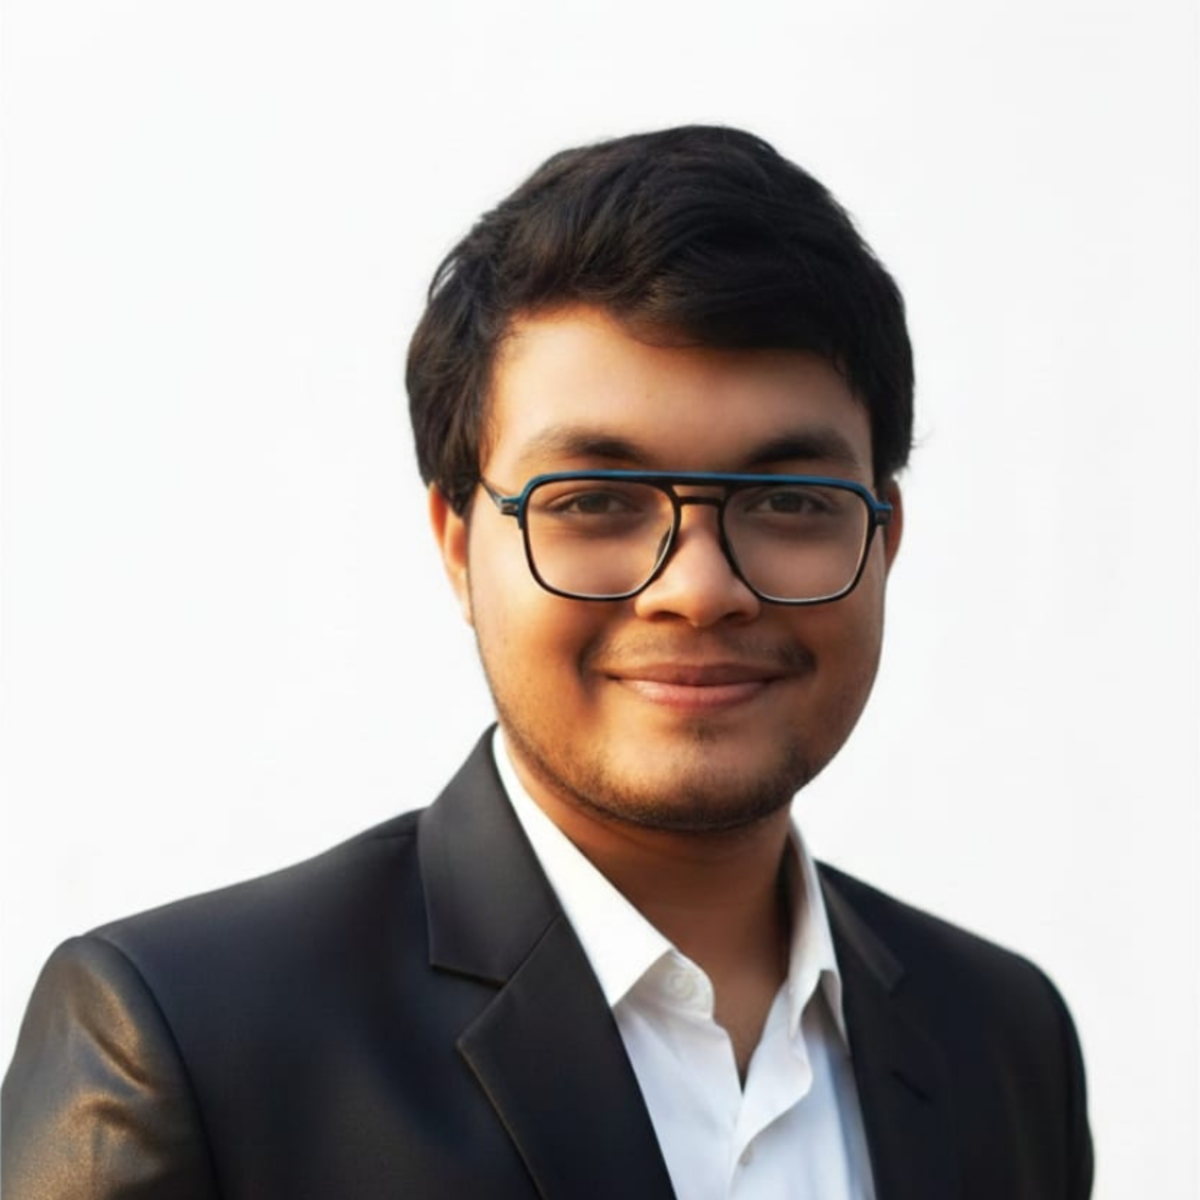
\includegraphics[width=64pt,height=76pt,keepaspectratio]{picture.jpg}}
\end{minipage}

\vspace{10pt}

%----------------------------------------------------------------------------------------
%	PROFESSIONAL SUMMARY
%----------------------------------------------------------------------------------------
\cvsection{Professional Summary}
\cvitem{Overview}{\textbf{Computer Science undergraduate specializing in Artificial Intelligence \& Machine Learning} at Adamas University, with research interests spanning healthcare AI, Edge AI, brain research \& neurotech, intelligent systems, and environmental data science. Experienced in developing machine learning pipelines for large-scale real-world datasets, building scalable software systems, and leading large-scale open-source engineering initiatives. Passionate about advancing reliable, scalable, and impactful intelligent systems for healthcare and environmental applications through the integration of research and software engineering.}

%----------------------------------------------------------------------------------------
%	RESEARCH INTERESTS
%----------------------------------------------------------------------------------------
\cvsection{Research Interests}
\cvitem{Healthcare \& Bio-AI}{AI for Asthma \& Respiratory Health, Brain Research, Neurotech \& Depression Mitigation}
\cvitem{Machine Learning}{Artificial Intelligence, Machine Learning, Edge AI \& TinyML, Explainable AI (XAI)}
\cvitem{Systems}{Distributed Systems, Cyber-Physical Systems, Intelligent Systems}
\cvitem{Data Science}{Environmental Data Science, Time Series Analysis \& Forecasting, Geospatial AI}

%----------------------------------------------------------------------------------------
%	EDUCATION
%----------------------------------------------------------------------------------------
\cvsection{Education}

\cventry{2024--2028}{Bachelor of Technology in Computer Science \& Engineering}{Specialization: Artificial Intelligence \& Machine Learning}{Adamas University}{Kolkata, India}{%
\textbf{CGPA:} \textbf{9.30 / 10.00} \\
\textbf{Relevant Coursework:} Machine Learning, Artificial Intelligence, Data Structures \& Algorithms, Operating Systems, Database Management Systems, Computer Networks, Probability \& Statistics, Linear Algebra.
}

\cventry{2019--2021}{Higher Secondary Education (Class XII)}{B.T. Road Govt. Spon. H.S. School}{Kolkata}{India}{%
\textbf{Score:} \textbf{89.6\%} \ \textperiodcentered\ \ \textbf{Stream:} Pure Science (Physics, Chemistry, Mathematics, Biology -- PCMB)
}

\cventry{2017--2019}{Secondary Education (Class X)}{B.T. Road Govt. Spon. H.S. School}{Kolkata}{India}{%
\textbf{Score:} \textbf{93.7\%}
}

%----------------------------------------------------------------------------------------
%	RESEARCH EXPERIENCE
%----------------------------------------------------------------------------------------
\cvsection{Research Experience}

\cventry{Aug 2025 -- Nov 2025}{Lead ML Researcher}{Urban Air Quality Analytics}{Adamas University}{Kolkata, India}{%
\begin{itemize}
    \item \textbf{Dataset \& Preprocessing}: Curated continuous ambient air quality monitoring (CAAQMS) datasets across 13 stations; engineered pipeline with timestamp alignment, missing value imputation, and Hampel / IQR outlier filtering.
    \item \textbf{ML Benchmarking}: Evaluated Linear Regression, Decision Trees, SVR, XGBoost, and LSTMs; achieved optimal non-linear predictive mapping with Random Forest modeling VOC, $\mathrm{NO}_x$, and $\mathrm{O}_3$ concentrations.
    \item \textbf{Atmospheric Dynamics}: Analyzed diurnal trends, seasonal heatmaps, and ozone-titration photochemical dynamics under meteorological parameters.
    \item \textbf{Publication}: Co-authored research manuscripts under preparation for journal submission.
\end{itemize}
}

%----------------------------------------------------------------------------------------
%	PUBLICATIONS & MANUSCRIPTS
%----------------------------------------------------------------------------------------
\cvsection{Publications \& Manuscripts}

\cvitem{Manuscript in Preparation (2026)}{%
Argha Kamal Guha, \textbf{Saptarshi Sadhu}, Chirag Deb. \textit{"Ozone Photochemical Regimes and Particulate Transport in Kolkata and Howrah."} Manuscript in preparation, 2026.
}

\cvitem{Manuscript in Preparation (2026)}{%
Argha Kamal Guha, \textbf{Saptarshi Sadhu}, Susmit Bagchi, Chirag Deb. \textit{"A Statistical Distribution, Spatial Autocorrelation, and Recurrent Neural Network Framework for High-Resolution Air Quality Forecasting in the Kolkata--Howrah Metropolitan Airshed, India."} Manuscript in preparation, 2026.
}

\cvitem{Manuscript in Preparation (2026)}{%
Argha Kamal Guha, Enubothula Bala Mani, Piyush Raj, Navnit Kumar, \textbf{Saptarshi Sadhu}, Snehamanju Basu. \textit{"Assessment of Particulate and Gaseous Pollution and its Statistical Distribution: A Case Study of Urban Area of Barrackpore Municipality."} Manuscript in preparation, 2026.
}

\cvitem{Manuscript in Preparation (2026)}{%
Co-authors, \textbf{Saptarshi Sadhu} (4th Author). \textit{"Enhancing Micro Electrochemical Spark Machining of Exotic Non-Ferrous Materials through On-Process Electrolyte Sonication."} Manuscript in preparation, 2026.
}

%----------------------------------------------------------------------------------------
%	OPEN SOURCE LEADERSHIP
%----------------------------------------------------------------------------------------
\cvsection{Open Source Leadership}

\cventry{Mar 2026 -- Pres.}{Lead Maintainer \& Systems Architect}{EaseMotion CSS Framework}{\href{https://github.com/SAPTARSHI-coder/EaseMotion-css}{GitHub Repository}}{}{%
\begin{itemize}
    \item \textbf{Global \& National Contributor Rank}: Ranked \textbf{\#3 top private committer in India} (\href{https://committers.top/india_private}{Committers.top Private}) and \textbf{\#2 active in commits} (\href{https://committers.top/india_public}{Committers.top Public}).
    \item \textbf{Large-Scale Project Maintenance}: Orchestrated codebase evolution under GirlScript Summer of Code (GSSoC) 2026, scaling framework to \textbf{21,587 merged pull requests, 54,166 commits, and 642 contributors} in 50 days (avg 496 PRs/day).
    \item \textbf{Automated Anti-Spam Architecture}: Deployed a \textbf{Honeypot Sandbox Relocation System} to automatically route, isolate, and audit point-farming spam folders.
    \item \textbf{CI/CD Optimization}: Engineered GitHub Actions pipelines with caching and REST/GraphQL API optimizations, cutting validation runtime from \textbf{3 minutes to under 25 seconds} per PR.
\end{itemize}
}

%----------------------------------------------------------------------------------------
%	TECHNICAL PROJECTS
%----------------------------------------------------------------------------------------
\cvsection{Technical Projects}

\cventry{Full-Stack}{CivicIssue Dashboard}{\href{https://github.com/SAPTARSHI-coder/civicissue-dashboard}{GitHub Repository}}{MVC Architecture}{}{%
Developed a full-stack MVC application integrating bcrypt password hashing, session management, input validation, and protected routing for city-level civic complaint reporting.
}

\cventry{JavaScript}{Multi-Source Weather Forecast App}{\href{https://github.com/SAPTARSHI-coder/Weather-App}{GitHub Repository}}{REST API \& Async JS}{}{%
Built an asynchronous weather forecasting tool featuring a backend proxy server to prevent API rate-limiting, custom caching layers, and automated fallback endpoints.
}

\cventry{AI Platform}{Techtonics -- AI Assisted Coding Platform}{\href{https://github.com/SAPTARSHI-coder/Techtonics}{GitHub Repository}}{AI API Integration}{}{%
Developed an interactive learning platform connecting real-time AI tutor APIs to guide beginners with step-by-step logic breakdown and syntax diagnostics.
}

\cventry{Web App}{Personal Portfolio Website}{\href{https://github.com/SAPTARSHI-coder/Portfolio}{GitHub Repository}}{Responsive Web}{}{%
Designed and developed a personal portfolio showcasing projects and technical skills with responsive design across devices, integrated project links, and optimized SEO.
}

%----------------------------------------------------------------------------------------
%	TECHNICAL SKILLS
%----------------------------------------------------------------------------------------
\cvsection{Technical Skills}

\cvitem{Programming}{Python, C, C++, Java, JavaScript, SQL, LaTeX}
\cvitem{Machine Learning}{Scikit-Learn, Pandas, NumPy, Matplotlib, Seaborn, Feature Engineering, Model Evaluation, Regression, Classification, Time Series, Explainability (SHAP)}
\cvitem{Web}{React.js, Node.js, Express.js, HTML5, CSS3, Tailwind CSS, Bootstrap, EJS, REST APIs}
\cvitem{Databases \& DevOps}{MongoDB, MySQL, Supabase, Git, GitHub Actions, CI/CD Automation, Linux}
\cvitem{GIS}{Google Earth Engine, QGIS, Raster Analysis, NDVI, LST, Satellite Analytics}

%----------------------------------------------------------------------------------------
%	AWARDS & ACHIEVEMENTS
%----------------------------------------------------------------------------------------
\cvsection{Awards \& Achievements}

\cvitem{July 2026}{\textbf{ACM Summer School at IISC Bangalore}:Selected to attend the summer school at IISC Bangalore}
\cvitem{May 2026}{\textbf{Google Student Ambassador (2026)}: Selected campus representative to lead technical programs and AI workshops.}
\cvitem{April 2026}{\textbf{4th Place Coding Premier League}: Algorithmic problem-solving finishes.}
\cvitem{February 2026}{\textbf{AWS College Showcase}: Selected among top 7 university teams for cloud innovation.}
\cvitem{June - July 2025}{\textbf{LetsUpgrade}: Campus Ambassador}
\cvitem{Mar 2025}{\textbf{Clash of Coders 2.0 Finalist }: Algorithmic problem-solving finishes and Software making brainstorming competition.}
\cvitem{HackerRank}{\textbf{4-Star Rating in C} and \textbf{3-Star Rating in C++ / Problem Solving} on HackerRank platform.}

%----------------------------------------------------------------------------------------
%	LEADERSHIP & SERVICE
%----------------------------------------------------------------------------------------
\cvsection{Leadership \& Service}

\cventry{Apr 2026 -- Pres.}{Publicity Chair}{ACM Student Chapter, Adamas University}{Kolkata}{India}{%
Architected promotional campaigns driving 30\% growth in chapter attendance, managed social media channels, and coordinated technical guest lectures.
}

\cventry{Mar 2026 -- Pres.}{Student Coordinator}{IETE Student Chapter, Adamas University}{Kolkata}{India}{%
Spearheaded student events, maintained membership databases, and served as primary student-faculty liaison.
}

\cventry{Oct 2025 -- Pres.}{Class Representative (CR)}{Department of CSE, Adamas University}{Kolkata}{India}{%
Advocated academic resources and resolved concerns for 60+ computer science undergraduates.
}

\cventry{Feb 2026}{Team Leader}{AI Impact Summit Buildathon (HCL GUVI)}{Kolkata}{India}{%
Led development of a multilingual AI vs. human text detection system across 5 languages, maintaining 6+ days continuous uptime via ngrok.
}

\cventry{Sep 2024 \& Sep 2025}{Team Leader}{Smart India Hackathon (SIH) 2024 \& 2025}{Adamas University}{Kolkata}{India}{%
Directed project timelines, brainstorming sessions, and solution design across two SIH editions.
}

%----------------------------------------------------------------------------------------
%	ACADEMIC EXPOSURE
%----------------------------------------------------------------------------------------
\cvsection{Academic Exposure}

\cvitem{Quantum Lab, 16th April 2026}{\textbf{TCG CREST Quantum Lab Visit (CQuERE)}: Academic visit exploring quantum computing algorithms and experimental research.}
\cvitem{Data Centre, 16th October 2025}{\textbf{CTRLS Enterprise Data Centre Visit}: Industrial visit gaining direct exposure to enterprise server infrastructure and cloud architecture.}

%----------------------------------------------------------------------------------------
%	CERTIFICATIONS
%----------------------------------------------------------------------------------------
\cvsection{Certifications}

\cvitem{2026}{\textbf{AI Impact Summit Buildathon Certificate} --- HCL GUVI}
\cvitem{2025}{\textbf{Urban Vision Hackathon 2025 Certificate of Achievement} --- Ministry of Education, Govt. of India, Organised by IISC Bangalore}
\cvitem{2025}{\textbf{Full Stack Web Development Training} --- DevTown}
\cvitem{2025}{\textbf{Data Structures \& Algorithms using C++} --- DevTown}
\cvitem{2025}{\textbf{Competitive Programming Course} --- DevTown}

%----------------------------------------------------------------------------------------
%	LANGUAGES
%----------------------------------------------------------------------------------------
\cvsection{Languages}

\cvitem{Proficiency}{\textbf{English} (Upper Intermediate Proficient, B2) \ \textperiodcentered\ \ \textbf{Bengali} (Native) \ \textperiodcentered\ \ \textbf{Hindi} (Proficient, C2) \ \textperiodcentered\ \ \textbf{German} (Beginner, A1)}

\end{document}
